
\subsection{Maximum Likelihood}

\begin{frame}
\thetitle{Learning with Maximum Likelihood}
 Objective: Find model parameters $\theta$ that maximize the likelihood of the data,
        
    \[ \theta^* = \argmax_\theta\sum_{n=1}^N \log p(x^{(n)} \param \theta) \]

    %\begin{itemize}
    %\item (Our core focus in this tutorial.) 
    %\end{itemize}
    %\begin{itemize}
    %   \item Dominant framework in probabilistic modeling. 
       %Intuition: find model parameters that maximize the probability of seeing the observed data.
    %    \item Minimizes the KL-divergence with data dist.
    %    $p_\star(x)$,
    %    \[\argmin_\theta \ \KL[p_\star(x) \Vert p(x \param \theta)] = \E_{p_\star(x)}\Big[\log %\frac{p_\star(x)}{p(x \param \theta)} \Big]\]
    %    \item Enjoys many nice statistical properties: consistency, asymptotic normality, etc.
    %\end{itemize}
\end{frame}

\begin{frame}
\thetitle{Learning Deep Models}
    \[  L(\theta) =  \sum_{n=1}^N \log p(x^{(n)} \param \theta)  \]
        \begin{center}
\begin{tikzpicture}
% nodes
%\node (dots) {$\ldots$};%
\node[obs] (x1) {$x$};%
 \node[const, below=1cm of x1] (pi) {$\theta$};
% plate
 \plate {plate1} {(x1)} {$N$}; %
% edges
 %\edge[bend left] {x1.south} {xT.south};
 \edge {pi} {x1.south};

 %\draw[->]
 %(dots) edge[bend right] node [right] {} (xT);
 
\end{tikzpicture}
\end{center}
    \begin{itemize}
        \item Dominant framework is gradient-based optimization: 
        \[ \theta^{(i)} = \theta^{(i-1)} + \eta \nabla_\theta L(\theta)\]
        \item $\nabla_\theta L(\theta)$ calculated with backpropagation.
        \item Tactics: mini-batch based training, adaptive learning rates \citep{duchi2011,Kingma2015}.
    \end{itemize}
\end{frame}

\begin{frame}
\thetitle{Learning Deep Latent-Variable Models: Marginalization}
Likelihood requires summing out the latent variables,
    \[p(x^{} \param \theta) = \sum_{z \in \mathcal{Z}} p(x^{}, z \param \theta)\ \  \text{(= $\int p(x, z \param \theta) dz$ if continuous $z$)} \]
    \pause
    
 In general, \textbf{hard to optimize} log-likelihood for the training set,
\[  L(\theta) =  \sum_{n=1}^N \log \sum_{z \in \mathcal{Z}} p(x^{(n)} , z \param \theta)  \]
\begin{center}
        \begin{tikzpicture}
          %\tikz{
        % nodes
         \node[obs] (x1) {$x^{(n)}$};%
         \node[latent, above = of x1] (z) {$z^{(n)}$}; %
         %\node[const, above=of z] (mu) {$\bmu$};
         \node[const, left = of z] (pi) {$\theta$};
         \plate {plate1} {(x1)(z)} {$N$}; %
         \edge {z} {x1};
         \edge {pi.east} {x1};
         \edge {pi.east} {z};

         %}
         
         \end{tikzpicture}
\end{center}
%\begin{itemize}
%\item In general, \textbf{hard to optimize}. Either requires enumeration of $\mathcal{Z}$
%or computation of integral in continuous case. Key focus of next section. 
%\end{itemize}

\end{frame}

%\begin{frame}
%\thetitle{Optimizing Marginal Likelihood in a Deep Model}
%\[  L(\theta) =  \sum_{n=1}^N \log \sum_{z \in \mathcal{Z}} p(x^{(n)} , z \param \theta)  \]

%\begin{itemize}
%\item In general, this objective is hard to optimize. Either requires enumeration of $\mathcal{Z}$
%or computation of integral in continuous case. 

%\item (However can maximize directly in many special cases. Discussed in next section.)
%\end{itemize}
%\end{frame}

%\begin{frame}
%\thetitle{Direct Optimization}
%\[  L(\theta) =  \sum_{n=1}^N \log \sum_{z \in \mathcal{Z}} p(x^{(n)} , z \param \theta)  \]
%Is this hard to optimize?
%\begin{itemize}
%    \item In many cases, it's not! If $\mathcal{Z}$ is not large, can simply enumerate. (Even parallelizes on GPUs)
%    \item Or perhaps  $\sum_{z \in \mathcal{Z}} p(x, z \param \theta)$ factors to allow for dynamic programming (HMM/PCFG etc).
%\end{itemize}
%\end{frame}

%\begin{frame}
%\thetitle{Hard cases}
%\vspace{-3mm}
%\[  L(\theta) =  \sum_{n=1}^N \log \sum_{z \in \mathcal{Z}} p(x^{(n)} , z \param \theta)  \]
%\begin{itemize}
%    \item In general,
%    \[ p(x\param \theta) = \sum_{z \in \mathcal{Z}} p(x, z \param \theta)\]
%    is linear in $|\mathcal{Z}|$, which can be expensive or even exponentially large (e.g. trees).
%    \item In the continuous case, the integral 
%    \[ p(x \param \theta) = \int_\mathcal{Z} p(x, z \param \theta) dz \]
%    is tractable if prior $p(z \param \theta)$ is \textbf{conjugate} to the likelihood 
%    $p(x \given z \param \theta)$. Almost never the case with deep likelihood models.
%\end{itemize}
%\end{frame}

\subsection{ELBO}


\begin{frame}
\thetitle{Variational Inference}

High-level: decompose objective into \alert{lower-bound} and \structure{gap}. 

\begin{center}
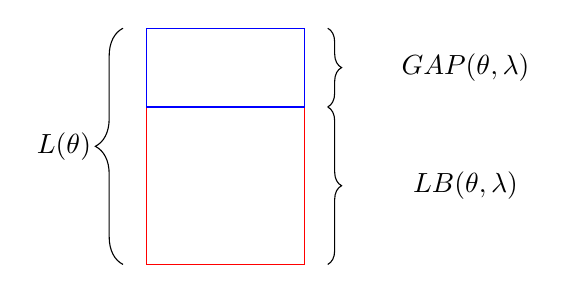
\begin{tikzpicture}
    \draw[decorate,decoration={brace,amplitude=10pt}] (-0.3, 0) -- node[xshift=-0.75cm]{$L(\theta)$} (-0.3, 3);
    
    \draw[red] (0, 0) rectangle (2, 2);
    \draw[blue] (0, 2) rectangle (2, 3);
    \draw[decorate,decoration={brace,amplitude=5pt}] (2.3, 2) -- node[xshift=1.75cm]{$\alert{\text{LB}}(\theta, \lambda)$} (2.3, 0);
    \draw[decorate,decoration={brace,amplitude=5pt}] (2.3, 3) -- node[xshift=1.75cm]{$\structure{\text{GAP}}(\theta, \lambda)$} (2.3, 2);
\end{tikzpicture}
\end{center}
\[ L(\theta) = \alert{\text{LB}}(\theta, \lambda) + \structure{\text{GAP}}(\theta, \lambda)\  \text{for\ some}\ \lambda \]
Provides framework for deriving a rich set of optimization algorithms.
\end{frame}

\begin{frame}
\thetitle{Marginal Likelihood: Variational Decomposition}

For any\footnote{Technical condition: $\text{supp}(q(z)) \subset \text{supp}(p(z \given x \param \theta))$} distribution $q(z\given x; \lambda)$ over $z$, 

\[ L(\theta) = \textcolor{red}{\E_{q}\Big[\log \frac{p(x, z \param \theta)}{q(z\given x \param\lambda)} \Big]} + \textcolor{blue}{\KL[q(z\given x \param \lambda)  \, \Vert \, p(z \given x \param \theta)]}\] 

\begin{center}
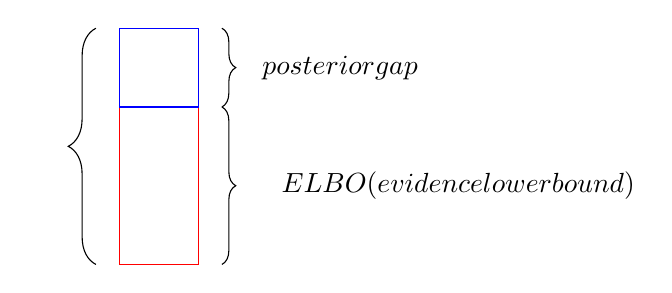
\begin{tikzpicture}
    \draw[decorate,decoration={brace,amplitude=10pt}] (-0.3, 0) -- node[xshift=-0.75cm]{} (-0.3, 3);
    
    \draw[red] (0, 0) rectangle (1, 2);
    \draw[blue] (0, 2) rectangle (1, 3);
    \draw[decorate,decoration={brace,amplitude=5pt}] (1.3, 2) -- node[xshift=3cm]{$\alert{\text{ELBO  (evidence lower bound) }}$} (1.3, 0);
    \draw[decorate,decoration={brace,amplitude=5pt}] (1.3, 3) -- node[xshift=1.5cm]{$\structure{\text{posterior gap}}$} (1.3, 2);
\end{tikzpicture}
\end{center}

%\begin{itemize}
%    \item The \alert{evidence lower bound} (ELBO)
%    \item The \structure{posterior gap}  
%\end{itemize}

Since KL is always non-negative, $L(\theta) \geq \ELBO(\theta, \lambda)$. 
\end{frame}

\begin{frame}
\thetitle{Evidence Lower Bound: Proof}
{
\begin{align*}
\log p(x \param \theta) &=\E_{q} \log p(x)  \quad  \text{\it (Expectation over $z$)} \\ \pause
&= \E_{q} \log \frac{p(x, z)}{p(z \given x)} \quad \text{\it (Mult/div by $p(z|x)$, combine numerator)}\\ \pause
&= \E_{q} \log \left( \frac{p(x, z )}{q(z\given x)} \frac{q(z\given x)}{p(z \given x)} \right) \quad \text{\it (Mult/div by $q(z|x)$)}\\ \pause
&= \E_{q} \log \frac{p(x, z )}{q(z\given x )}  + \E_{q}  \log \frac{q(z \given x)}{p(z \given x )}  \quad  \text{\it (Split Log)}\\ \pause
%&= \int q(z ) \log \frac{p(x, z \param \theta)}{q(z )} \, dz + \KL[q(z )  \, \Vert \, p(z \given x \param \theta)]  \\
&= \alert{\E_{q}  \log \frac{p(x, z \param \theta)}{q(z\given x;\lambda )}} + \structure{\KL[q(z \given x;\lambda)  \, \Vert \, p(z \given x \param \theta)]}  \\
%&= \ELBO(x, \theta, \lambda) \qquad \qquad  \, + \KL[q(z )  \, \Vert \, p(z \given x \param \theta)] 
\end{align*}
}
\end{frame}


%\begin{frame}
%\thetitle{Evidence Lower Bound}
%\begin{itemize}
%    \item For each $x^{(n)}$, let $q_n(z)$ be a distribution over $z$, i.e.
%    \[ q_n(z) : \mathcal{Z} \to \reals_{\ge 0}, \,\,\,\, \,\,\,\,\,\,\,\, \int_{\mathcal{Z}} q_n(z) dz = 1\]
%    \item Define the \textbf{evidence lower bound} (ELBO) for a single point as 
%    \[ \ELBO(\theta, q \param x) = \E_{q(z)}\Big[\log \frac{p(x, z \param \theta)}{q(z)} \Big]\]
%    \item Aggregate ELBO
%    \[ L(\theta, q_1, \dots, q_N) = \sum_{n=1}^N \ELBO(x^{(n)}, \theta, q_n)\]
%\end{itemize}
%\end{frame}

\begin{frame}
\thetitle{Evidence Lower Bound over Observations}
    \[ \ELBO(\theta, \lambda; x) = \E_{q(z)}\Big[\log \frac{p(x, z \param \theta)}{q(z\given x;\lambda)} \Big]\]
\begin{itemize}
    \item ELBO is a function of the generative model parameters, $\theta$, and the variational parameters, $\lambda$.
\end{itemize}
\begin{align*}
    \sum_{n=1}^N \log p(x^{(n)} \param \theta) &\ge \sum_{n=1}^N \ELBO(\theta, \lambda \param x^{(n)}) \\
    &= \sum_{n=1}^N \E_{q(z \given x^{(n)} \param \lambda)}\Big[\log \frac{p(x^{(n)}, z \param \theta)}{q(z \given x^{(n)} \param \lambda)} \Big] \\
    &= \ELBO(\theta, \lambda \param x^{(1:N)}) = \ELBO(\theta, \lambda)
\end{align*} 
\end{frame}


%\begin{frame}
%\thetitle{Evidence Lower Bound: Property 1}
%    \[ \ELBO(x, \theta, q) = \E_{q(z)}\Big[\log \frac{p(x, z \param \theta)}{q(z)} \Big]\]
%Property 1: If $\text{supp}(q(z)) \subset \text{supp}(p(z \given x \param \theta))$ then
%the ELBO lower bounds the log marginal likelihood for any $q(z)$, i.e.
%\[ \ELBO(x, \theta, q) \le \log p(x \param \theta) = \log \int_\mathcal{Z} p(x, z \param \theta) dz \]
%\end{frame}



%\begin{frame}
%\thetitle{Evidence Lower Bound: Property 2}
%Property 2: If $q(z) = p(z \given x \param \theta)$, then the bound is tight
%\begin{align*}
%    \ELBO(x, \theta, p(z \given x \param \theta)) &= \E_{p(z \given x \param \theta)}\Big[\log \frac{p(x, z \param \theta)}{p(z \given x \param \theta)} \Big] \\
%    &= \E_{p(z \given x \param \theta)}\Big[\log \frac{p(x \param \theta)p(z \given x \param \theta)}{p(z \given x \param \theta)} \Big] \\
%    &= \E_{p(z \given x \param \theta)}[\log p( x \param \theta)]  \\
%    &= \log p( x \param \theta)
%\end{align*}
%\end{frame}





\begin{frame}
\thetitle{ Setup: Selecting Variational Family}
\begin{itemize}
    
    \item Just as with $p$ and $\theta$, we can select any form of $q$ and $\lambda$ that satisfies ELBO conditions. 
    \item Different choices of $q$ will lead to different algorithms.
    \item We will explore several forms of $q$: 
    \begin{itemize}
        \item Posterior
        \item Point Estimate / MAP
        \item Amortized
        \item Mean Field (later)
    \end{itemize}
\end{itemize}
\end{frame}

\begin{frame}
\thetitle{Example Family : Full Posterior Form}
\begin{center}
    \begin{tikzpicture}
% nodes
 \node[latent] (zl) {$z^{(n)}$};%
 %\node[const, below=of zl] (xl) {$x^{(n)}$};%
 %\node[obs, right=1cm of dots] (xT) {$x_T^{(n)}$};%
 \node[const, below=of zl] (lambda) {$\lambda^{(n)}$};
% plate
 \plate {plate1} {(zl)(lambda)} {$N$}; %
 \edge{lambda}{zl};
 
 \begin{scope}[xshift=5cm]
%\node (dots) {$\ldots$};%
 %\node[obs, right=1cm of dots] (xT) {$x_T^{(n)}$};%
 \node[latent] (z) {$z^{(n)}$}; %
 \node[obs, below=of z] (x1) {$x^{(n)}$};%
% \node[const, above=of z] (mu) {$\bmu$};
 \node[const, right= of x1] (pi) {$\theta$};
 
% plate
 \plate {plate1} {(x1)(z)} {$N$}; %
% edges
 \edge {z} {x1};
 %\edge {mu} {z};
 \edge {pi} {x1, z};
 \end{scope}
 \draw[dashed] (zl) --node [yshift=0.2cm] {$\KL(q(z \given x )\  ||\  p(z \given x))$} (z);
\end{tikzpicture}
\end{center}
$\lambda = [\lambda^{(1)}, \dots, \lambda^{(N)}]$ is a concatenation of local variational parameters $\lambda^{(n)}$, e.g.
    \[ q(z^{(n)} \given x^{(n)} \param \lambda) = q(z^{(n)} \given x^{(n)} \param \lambda^{(n)}) =   \mathcal{N}(\lambda^{(n)} , 1) \]
\end{frame}


\begin{frame}
\thetitle{Example Family: Amortized Parameterization \citep{Kingma2014}}
\begin{center}
    \begin{tikzpicture}
% nodes
 \node[latent] (zl) {$z^{(n)}$};%
 \node[const, below=of zl] (xl) {$x^{(n)}$};%
 %\node[obs, right=1cm of dots] (xT) {$x_T^{(n)}$};%
 \node[const, above=of zl] (lambda) {$\lambda$};
% plate
 \plate {plate1} {(zl)(xl)} {$N$}; %
 \edge{lambda}{zl};
 \edge{xl}{zl};
 
 \begin{scope}[xshift=5cm]
%\node (dots) {$\ldots$};%
 %\node[obs, right=1cm of dots] (xT) {$x_T^{(n)}$};%
 \node[latent] (z) {$z^{(n)}$}; %
 \node[obs, below=of z] (x1) {$x^{(n)}$};%
% \node[const, above=of z] (mu) {$\bmu$};
 \node[const,  right= of x1] (pi) {$\theta$};
 
% plate
 \plate {plate1} {(x1)(z)} {$N$}; %
% edges
 \edge {z} {x1};
 %\edge {mu} {z};
 \edge {pi} {x1, z};
 \end{scope}
 \draw[dashed] (zl) --node [yshift=0.2cm] {$\KL(q(z \given x) || p(z \given x))$} (z);
\end{tikzpicture}
\end{center}
$\lambda$ parameterizes a global network (encoder/inference network) that is run over $x^{(n)}$
    to produce the local variational distribution, e.g.
    \[ q(z^{(n)} \given x^{(n)} \param \lambda) = \mathcal{N}(\mu^{(n)} , 1), \,\, \,\,\,\,\,\,\,\,\,\,\, \mu^{(n)} = \enc(x^{(n)} \param \lambda)\]
\end{frame}